\section{ΣΥΝΑΛΛΑΓΕΣ ΣΕ ΣΥΣΤΗΜΑΤΑ ΔΕΔΟΜΕΝΩΝ ΜΕΓΑΛΗΣ ΚΛΙΜΑΚΑΣ}
    Η συλλογή με τίτλο "\textit{Transactions on Large-Scale Data and Knowledge Centered Systems XXIV}" περιλαμβάνει ένα σύνολο από δημοσιεύσεις. \cite{TransactionsonLargeScale}

    Περιλαμβάνονται τα εξής:
    \paragraph{Reflective Constraint Writing: A Symbolic Viewpoint of Modeling Languages}
        Παρουσιάζεται ένας τρόπος για την επέκταση των object constraint γλωσσών (περιγράφουν κανόνες που ισχύουν σε UML μοντέλα) μέσω του reflection, επιτρέποντας έτσι τα metadata να είναι διαθέσιμα στο επίπεδο του αντικειμένου.

    \paragraph{PPP-Codes for Large-Scale Similarity Searching}
        Παρουσιάζεται ένας τρόπος για να αντιμετωπιστεί η δυσκολία του αποτελεσματικού εντοπισμού παρόμοιων αντικειμένων σε μεγάλους χώρους αναζήτησης.
        Επιτυγχάνεται μέσω μιας αναζήτησης δύο φάσεων που χρησιμοποιεί μια νέα δομή δεδομένων που ονομάζεται δείκτης PPP-Code, ο οποίος υπολογίζεται ανεξάρτητες κατατάξεις (rankings) χρησιμοποιώντας μια συνάρτηση απόστασης και συγκεντρώνει αυτές τις κατατάξεις αυξάνοντας την αποτελεσματικότητα της αναζήτησης.

    \paragraph{Solving Data Mismatches in Bioinformatics Workflows by Generating Data Converters}
        Λόγω της ετερογένειας των δεδομένων στη βιοπληροφορική, συχνά παρουσιάζονται αναντιστοιχίες (mismatches) μεταξύ των εισόδων και των εξόδων σε διαφορετικά λογισμικά και υπηρεσίες, κάτι που καθιστά δύσκολη την δουλειά των επιστημόνων.
        Μέχρι πρότινος, ένας τρόπος για την ενοποίηση των δεδομένων είναι οι slims μετατροπείς, που είναι χρονοβόρο να τους γράψεις με το χέρι, και όταν δημιουργούνται αυτόματα δεν είναι αποτελεσματικοί.

        Το άρθρο παρουσιάζει ένα νέο τρόπο για τη συστηματική μετατροπή των εξόδων σε εισόδους, χρησιμοποιώντας ένα σύστημα κανόνων παρόμοιο με το XML Schema.

    \paragraph{A Framework for Sampling-Based XML Data Pricing}
        Παρουσιάζεται ένα framework για την τιμολόγηση XML εγγράφων, θέτοντας ένα βάρος σε κάθε έγγραφο.

    \paragraph{kdANN+: A Rapid AkNN Classifier for Big Data}
        Παρουσιάζεται ο kdANN+, ένας αποδοτικός ταξινομητής K-Nearest-Neighbour, σχεδιασμένος για big data εφαρμογές.
        Παρουσιάζονται αλγόριθμοι που βελτιώνουν την ταχύτητα και την ακρίβεια της ταξινόμησης (classification) σε μεγάλα σύνολα δεδομένων, κάνοντάς τον κατάλληλο για real-time εφαρμογές.

    \paragraph{Optimizing Inter-data-center Large-Scale Database Parallel Replication with Workload-Driven Partitioning}
        Εισάγεται μια partitioning στρατηγική με σκοπό τη βελτιστοποίηση παράλληλης αντιγραφής σε distributed big-data βάσεις δεδομένων.

    \paragraph{Anonymization of Data Sets with NULL Values}
        Διερευνώνται μεθόδους για την ανωνυμοποίηση συνόλων δεδομένων που περιλαμβάνουν NULL τιμές.

    \noindent Θα εστιάσουμε στο "Solving Data Mismatches in Bioinformatics Workflows by Generating Data Converters".

    \subsection{Αυτόματος μετατροπέας}
        Παρουσιάζεται ένας αυτόματος μετατροπέας που βασίζεται σε έναν μηχανισμό κανόνων που ανιχνεύει αν υπάρχει μετατρεψιμότητα μεταξύ διαφορετικών τύπων δεδομένων.

        Ορίζεται ένα σύνολο τύπων αναπαράστασης που βασίζονται σε type constructors, όπου ο καθένας τους θέτει ένα σύνολο από XML τιμές.
        Παραδείγματα κανόνων μετατρεψιμότητας είναι: \texttt{PRIMITIVE}, \texttt{TAGCHANGE}, \texttt{TAGREMOVAL}, \texttt{EMPTY}, \texttt{CONCAT}, \texttt{LEFTSELECTION}, \texttt{MAP} και άλλοι.
        Αυτοί δημιουργούν αντίστοιχες συναρτήσεις που μετατρέπουν τις εισόδους σε XML:

        \begin{figure}[h!] \noindent\centering
            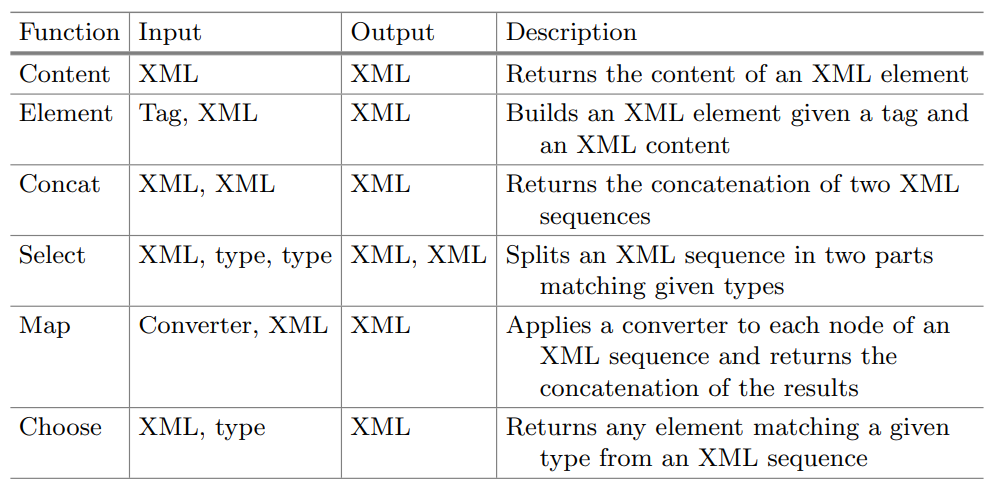
\includegraphics[scale=0.7]{img/Converter}
            \caption{Σύνολο συναρτήσεων \cite{TransactionsonLargeScale}}
        \end{figure}

        Όταν εντοπιστεί η σχέση μεταξύ των τύπων δεδομένων, το σύστημα δημιουργεί αυτόματα τους κατάλληλους μετατροπείς.
        Οι μετατροπείς ελέγχονται για τη βιολογική εγκυρότητά τους, και εν τέλει ενσωματώνονται στο workflow των ερευνητών, επιτρέποντας την απρόσκοπτη ροή δεδομένων μεταξύ διαφορετικών υπηρεσιών.
